% LREC-COLING 2024 Example; 
% LREC Is now using templates similar to the ACL ones. 
\documentclass[10pt, a4paper]{article}

\usepackage{lrec-coling2024} % this is the new style

\usepackage{fontspec}
\setmainfont{Arial}
\usepackage{listings}

\usepackage{natbib}
\usepackage{multibib}
\makeatletter
%\def\@mb@citenamelist{cite,citep,citet,citealp,citealt,citepalias,citetalias}
\makeatother
\newcites{languageresource}{~}
\renewcommand{\refname}{{}}
\usepackage{graphicx}
\usepackage{tabularx}
\usepackage{soul}
% for eps graphics
%%% References and Labels
%%% Reference labels without a punctuation 
% courtesy of Marc Schulder , uni Hamburg ****************
\usepackage{titlesec}
%\titleformat{\section}{\normalfont\large\bf\center}{\thesection.}{1em}{}
\titleformat{\section}{\normalfont\large\bfseries\center}{\thesection.}{1em}{}
\titleformat{\subsection}{\normalfont\SmallTitleFont\bfseries\raggedright}{\thesubsection.}{1em}{}
\titleformat{\subsubsection}{\normalfont\normalsize\bfseries\raggedright}{\thesubsubsection.}{1em}{}
\renewcommand\thesection{\arabic{section}}
\renewcommand\thesubsection{\thesection.\arabic{subsection}}
\renewcommand\thesubsubsection{\thesubsection.\arabic{subsubsection}}
%  ed 

\usepackage{microtype}
\usepackage{todonotes}
\usepackage{booktabs}
\usepackage{paralist}
\usepackage{colortbl}

\usepackage{xcolor}
\usepackage{hyperref}
 \definecolor{darkblue}{rgb}{0, 0, 0.5}
  \hypersetup{colorlinks=true, citecolor=darkblue, linkcolor=darkblue, urlcolor=darkblue}

\usepackage{xstring}

\usepackage{color}

\newcommand{\secref}[1]{\StrSubstitute{\getrefnumber{#1}}{.}{ }}

\title{Are Sounds Sound for the Reconstruction of Language Trees? Comparing Lexical Cognates and Sound Correspondences in Bayesian Phylogenetic Inference}

\name{} 

\address{ \\ \\ \\}% Affiliation1, Affiliation2, Affiliation3 \\
%         Address1, Address2, Address3 \\
%         author1@xxx.yy, author2@zzz.edu, author3@hhh.com\\
%         \{author1, author5, author9\}@abc.org\\}


\abstract{ In traditional studies on language evolution, scholars often emphasize the important role which sound laws and sound correspondences play in the task of reconstructing the phylogeny of a language family. However computational approaches have largely ignored the potential importance of sound laws and sound correspondences.  Most computational studies still employ lexical cognates as the major data when it comes to phylogenetic reconstruction in linguistics, although there are a few studies in which authors praise the benefits of comparing words at the level of sound sequences. Building on (a)~five diverse datasets from five different language families, and (b)~state-of-the-art methods for automated cognate and sound correspondence detection, we test, for the first time, the performance of sound-based versus cognate-based approaches to phylogenetic reconstruction.  Our results show that phylogenies reconstructed from lexical cognates tend to come closer to gold standard phylogenies than phylogenies reconstructed from sound correspondences.  \\ \newline \Keywords{sound correspondences, phylogenetic reconstruction lexical cognates}%
}

\begin{document}

\maketitleabstract%
%
\section{Introduction}

Although controversially discussed in the beginning \citep{Holm2007}, quantitative approaches tophylogenetic reconstruction based on Bayesian phylogenetic inference frameworks have now become broadly accepted in the field of comparative linguistics. This is reflected in more and more computer-based phylogenies that have been proposed for the world's largest language families---Dravidian \citep{Kolipakam2018}, Sino-Tibetan \citep{Sagart2019} and Indo-European \citep{bouckaert2012mapping}---and even fully automated workflows have shown to be quite robust \citep{rama2018automatic}.  While rarely practiced in the pre-computational past of historical linguistics, computing detailed phylogenies has now become one of the key tasks of studies on language evolution.


Although traditional scholars have started to accept computational language phylogenies as a new tool deserving its place in the large tool chain of comparative linguistics, scholars still express a lot of skepticism against the idea of most of the language phylogenies that have been proposed so far. One of the major reasons usually mentioned in this context is that phylogenetic approaches are usually based on cognate sets (sets of historically related words) identified in semantically aligned word lists. Since these \emph{cognate sets} reflect \emph{lexical data} only, many scholars mistrust them, given that lexical data are assumed to be much less stable than other aspects of languages~\cite{CampbellPoser2008}.
 
In classical historical linguistics, the data used for subgrouping are traditionally composed of small collections of so-called \emph{shared innovations} \citep{Dyen1953}. What counts as a shared innovation has itself never been well-defined in the literature, but the largest amount of data used by scholars is traditionally taken from sound correspondences or supposed sound change processes (compare, for example the data in \citealt[305]{Anttila1972}). Although it is controversially debated in the field \citep{Ringe2002,Dybo2008}, many classical linguists still emphasize that sound correspondences are largely superior to lexical data when it comes to subgrouping.

There have only been a few attempts to test how well quantitative approaches to phylogenetic reconstruction perform when using sound correspondences instead of lexical cognates \citep{Chacon2015a}. The main reason is that coding data to compute phylogenies from sound change data is very tedious even for a dataset with 20 languages.  Since coding data to compute phylogenies from sound change data is very tedious---specifically when working with more than just a few languages---there have only been a few attempts to test how well quantitative approaches to phylogenetic reconstruction perform when using sound correspondences instead of lexical cognates.
% \citep{Chacon2015a}. 

Building on the state-of-the-art methods for automatic cognate detection and phonetic alignment in historical linguistics \citep{List2016g}, combined with novel approaches for the inference of sound correspondence patterns in multilingual datasets \citep{List2019a} and customized solutions for phylogenetic reconstruction \citep{Rama2019} that have evolved into a new Python library for phylogenetic inference, we have been able to create a new workflow for phylogenetic reconstruction based on sound correspondence patterns.  With a new collection of five gold standard datasets, we test the workflow and compare it with alternative workflows based on lexical data alone. Our results indicate that sound correspondence patterns are far less suitable for the purpose of computer-based phylogenetic reconstruction than expected.

% The contributions\todo{The contributions as pointed by the reviewer.} of the paper are as followed:

% \begin{itemize}
%     \item A new implementation of phylogenetic inference software
%     \item automating sound-based representations and alignment
%     \item evaluating sound vs. lexical information
% \end{itemize}



%In this paper, we test if word aligned data be useful for phylogenetic inference for datasets ranging from dialects to languages. Do correspondence set algorithms reduce the ambiguity in the data which in turn can be used for inferring trees? Do multi-state characters perform better than binarized aligned data? In the face of uncertainty regarding the type of data, which level of data should be employed for phylogenetic inference? In the process of answering these questions, we developed and tested new phylogenetic inference software that uses a new algorithm known as serial tempering for navigating the tree space. We make all our data and code available with the paper.

\section{Background}\label{sec:motiv}

Much of the previous work on phylogenetic reconstruction using Bayesian phylogenetic inference~\cite{Kolipakam2018,Sagart2019,rama2018automatic} is based on cognate sets encoded as binary vectors, where the presence or absence of a language in a cognate set is coded as \textbf{0} or \textbf{1}, and phylogenetic trees are inferred by assuming that cognate sets evolve along a phylogenetic tree in the form of gain and loss processes (see Figure~\ref{fig:1}).

\begin{figure}[tb!]
    \centering
    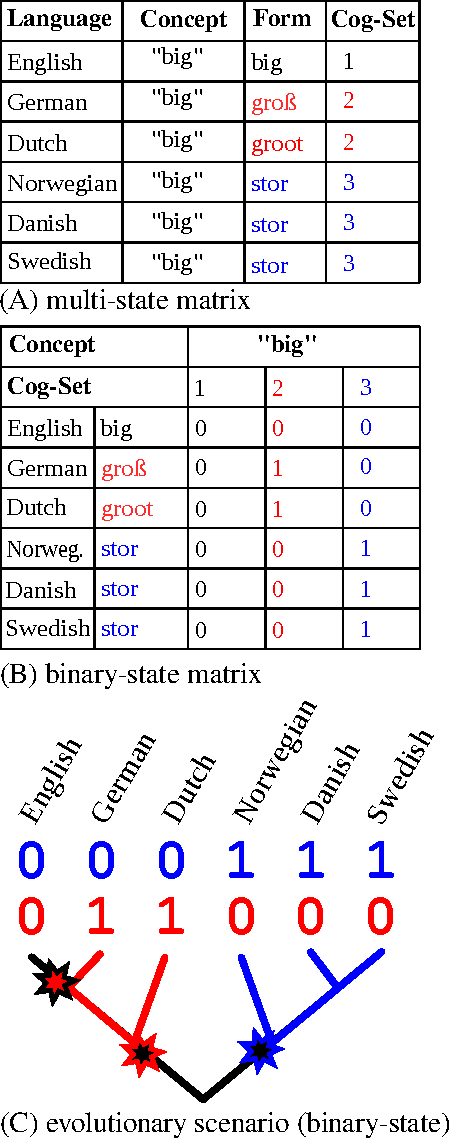
\includegraphics[width=0.4\textwidth]{figures/figure-1.pdf}
    \caption{Gain-loss processes derived from binary cognate vectors. A shows a wordlist in which
    cognate words are coded in multi-state fashion. B shows the corresponding binary coding. C shows
    how gain and loss processes are modeled on a phylogenetic tree.}\label{fig:1}
\end{figure}


The binary-state coding is the most frequently applied coding technique. Once assembled, binary state data can be modeled with binary state Continuous Time Markov Chain model (\emph{binary-CTMC}, \citealt{bouckaert2012mapping}), which allow gain and loss processes to occur an arbitrary number of times (details are given in Section~\ref{sec:BI}). While linguists tend to prefer these models intuitively, and there has been some debate about the limits of binary-state coding \citep{atkinson2006old,pagel2006estimating,List2016f}. It is well known that a multitude of processes can lead to \emph{lexical replacement}, including the typical transition through a synonymous phase in which a concept can be expressed by two or more word forms, and various derivation processes.

An alternative coding technique is to treat each concept in a wordlist as a single character and to allow for each character to have a range of different states.  In contrast, it is not clear what the \emph{transition} between multiple states is supposed to reflect when modeling character evolution on multi-state data with CTMC models. While multi-state models are rarely applied to lexical data, they have an immediate appeal for phonological data on sound correspondences and sound change processes, since it is well known that the sounds reflected in particular correspondence patterns can be numerous across larger language families.

The \textit{major contributions} of this study are:
\begin{inparaenum}[(1)]
\item we 
provide an automated workflow that 
allows
to infer cognates and correspondence patterns and analyze them with
the help of Bayesian phylogenetic inference methods, implemented in a new software package,
% \item we show how the workflow can be applied to
% standardized datasets, which were in part collected from existing studies and in part also specifically
% prepared for this study, and 
\item we show how the quality of phylogenetic reconstruction approaches based on sound correspondences can be compared to phylogenetic reconstruction based on lexical data, and in this way
\item we put the debate about the usefulness of sound-based as opposed to cognate-based phylogenies to the test.
\end{inparaenum}


As an early example for sound-based approaches to phylogenetic reconstruction, \citet{hruschka2015detecting} apply a CTMC model that allows transitions between a fixed number of sounds for detecting the important sound changes in a dataset consisting of etymologies across Turkic languages.
% The data themselves were extracted from multiple phonetic alignments that were created for each set of word forms assembled in a given etymology.  
The authors do not infer phylogenies from their data but rather use an established phylogeny (which are not readily available for many language families of the world) to infer branch lengths and transition probabilities between sounds in their data in order to detect sound changes at different time points in a time-calibrated family tree of Turkic. 
% Although the  with established family trees, the method is not 
% , but since data and code were not supplemented, replication is difficult to achieve, and it is also not clear where the upper bound of the number of sounds that may occur in a dataset lies.

\citet{Wheeler2015b} start from typical word lists (that would otherwise be used in phylogenetic reconstruction based on lexical data) and apply a parsimony-based algorithm that aligns words regardless if they are cognate or not, reconstructs a hypothetical ancestral word from the alignment, and seeks to infer the phylogeny that allows to explain the sequences by a minimal amount of assumed transitions \citep{Sankoff1975}. In a later study, \citet{Whiteley2019} apply the same approach to a dataset of Bantu languages. The method by \citet{Wheeler2015b} is linguistically flawed, since words are not assigned to cognate sets before aligning them. It is well known that there is a strict difference between regular sound change processes and processes resulting from lexical replacement \citep{Hall2010} and that even words that are cognate are not necessarily fully \emph{alignable}
\citep[10]{Schweikhard2020}.

% This is highly problematic, since it is well known that there is a strict difference between regular sound change processes and processes resulting from lexical replacement \citep{Hall2010} and that even words that are cognate are not necessarily fully \emph{alignable} \citep[10]{Schweikhard2020}.
 
\citet{Chacon2015a} start from manually extracted sound correspondence patterns for consonants in a dataset of 21 Tukanoan languages, to which proto-forms had also been added manually. Based on the sound correspondence patterns, they apply---similar to \citet{Wheeler2015b}---an algorithm that searches for the tree that provides the most parsimonious scenario for the evolution of the sounds. In contrast to \citet{Wheeler2015b}, however, they added specific constraints for the transitions from one sound to another sound, which were based on expert judgments for the Tukanoan language family. The approach by \citet{Chacon2015a}, finally, requires an enormous amount of preprocessing that runs the risk of leading to circular results, since proto-forms and major directions of sound change processes are required to be known in advance. While all approaches have their individual shortcomings, one of the largest shortcomings lies in the fact that it is very difficult to apply them. This is also witnessed by the fact that no additional studies have been carried out by other teams, although all the methods have been proposed years ago.


\section{Materials and Methods}

\subsection{Materials}

\begin{itemize}
\item describe datasets (table)
\item describe preprocessing 
\item describe binarization 
\end{itemize}


\subsection{Methods}

mostly gerhard on trees, etc.

\subsection{Evaluation}

mostly gerhard on trees

\subsection{Implementation}

Mattis + Gerhard

\section{Results}

Gerhard + mattis comments

\section{Discussion and Conclusion}

\section{Supplementary Material}



%LREC-COLING 2024 has long and short papers featuring substantial, original, and unpublished research in all aspects of natural language and computation, language resources (LRs) and evaluation, including spoken and sign language and multimodal interaction. Submissions are invited in five broad categories: (i) theories, algorithms, and models, (ii) NLP applications, (iii) language resources, (iv) NLP evaluation and (v) topics of general interest. Submissions that span multiple categories are particularly welcome.

%\begin{itemize}
%    \item{The paper is in A4-size format, that is 21 x 29.7 cm.}
%    \item{The text height is 24.7 cm and the text width 16.0 cm in two columns separated by a 0.6 cm space.}
%    \item {The font for the main body of the text must be Arial 10 pt with interlinear spacing of 11 pt.}
%    \item {The use of LREC-COLING2024.sty will ensure the good formatting.}
%    \item You must use \textbf{\texttt{XeTeX}} or \textbf{\texttt{LuaTeX}}
%\end{itemize}




\bibliographystylelanguageresource{lrec_natbib}
\bibliographylanguageresource{languageresource}

\bibliographystyle{lrec_natbib}
\bibliography{languageresource}

\newpage
\appendix

\section{Appendix: How to Produce the \texttt{.pdf}}%
\label{sec:append-how-prod}

\paragraph{Submissions may be of three types:}

\begin{itemize}
\item Regular long papers - up to eight (8) pages maximum,* presenting substantial, original, completed, and unpublished work.
\item Short papers - up to four (4) pages,\footnote{Excluding any number of additional pages for references, ethical consideration, conflict-of-interest, as well as data and code availability statements.} describing a small, focused contribution, negative results, system demonstrations, etc.
\item  Position papers - up to eight (8) pages,* discussing key hot topics, challenges and open issues, and cross-fertilization between computational linguistics and other disciplines.
\end{itemize}

Upon acceptance, final versions of long papers will be given one
additional page – up to nine (9) pages of content plus unlimited pages for acknowledgments and references – so that reviewers’ comments can be considered. Final versions of short papers may have up to five (5) pages, plus unlimited pages for acknowledgments and references. All figures and tables that are part of the main text must fit within these page limits for long and short papers.

Papers must be of original, previously-unpublished work. Papers must be \textbf{anonymized to support double-blind reviewing}. Submissions, thus, must not include authors’ names and affiliations. The submissions should also avoid links to non-anonymized repositories: the code should be either submitted as supplementary material in the final version of the paper or as a link to an anonymized repository (e.g., Anonymous GitHub or Anonym Share). Papers that do not conform to these requirements will be rejected without review.

\section{Final Paper}

Each final paper should be submitted online. The fully justified text should be formatted according to LREC-COLING2024 style as indicated for the Full Paper submission.

As indicated above, the font for the main body of the text should be Times  New Roman 10 pt with interlinear spacing of 11 pt. Papers must be between 4 and 8 pages long, including figures (plus more pages for references if needed), regardless of the presentation mode (oral or poster).

\subsection{General Instructions for the Final Paper}

The unprotected PDF files will appear in the online proceedings directly as received. \textbf{Do not print the page number}.

\section{Page Numbering}

\textbf{Please do not include page numbers in your Paper.} The definitive page numbering of papers published in the proceedings will be decided by the Editorial Committee.

\section{Headings / Level 1 Headings} 

Level 1 Headings should be capitalised in the same way as the main title, and centered within the column. The font used is Arial 12 pt bold. There should also be a space of 12 pt between the title and the preceding section and 3 pt between the title and the following text.

\subsection{Level 2 Headings}

The format of Level 2 Headings is the same as for Level 1 Headings, with the font Arial 11 pt, and the heading is justified to the left of the column. There should also be a space of 6 pt between the title and the preceding section and 3 pt between the title and the following text.

\subsubsection{Level 3 Headings}%
\label{level3H}

The format of Level 3 Headings is the same as Level 2, except that the font is Arial 10 pt, and there should be no space left between the heading and the text as in~\ref{level3H}. There should also be a space of 6 pt between the title and the preceding section and 3 pt between the title and the following text.

\section{Citing References in the Text}

\subsection{Bibliographical References}


\begin{table}
\centering
\begin{tabular}{lll}
\hline
\textbf{Output} & \textbf{natbib command} & \textbf{Old command}\\
\hline
%\citep{Eco:1990} & \verb|\citep| & \verb|\cite| \\
%\citealp{Eco:1990} & \verb|\citealp| & no equivalent \\
%\citet{Eco:1990} & \verb|\citet| & \verb|\newcite| \\
%\citeyearpar{Eco:1990} & \verb|\citeyearpar| & \verb|\shortcite| \\
\hline
\end{tabular}
\caption{\label{citation-guide} Citation commands supported by the style file. The style is based on the natbib package and supports all natbib citation commands. It also supports commands defined in previous style files for compatibility.}
\end{table}

Table~\ref{citation-guide} shows the syntax supported by the style files. We encourage you to use the natbib styles.
You can use the command \verb|\citet| (cite in text) to get ``author (year)'' citations, like this citation to a paper by %\citet{CastorPollux-92}. You can use the command \verb|\citep| (cite in parentheses) to get ``(author, year)'' citations \citep{CastorPollux-92}. You can use the command \verb|\citealp| (alternative cite without parentheses) to get ``author, year'' citations, which is useful for using citations within parentheses (e.g. \citealp{CastorPollux-92}).

When several authors are cited, those references should be separated with a semicolon: %\cite{Martin-90,CastorPollux-92}. When the reference has more than three authors, only cite the name of the first author followed by ``et. al.'', e.g. \cite{Superman-Batman-Catwoman-Spiderman-00}.

\subsection{Language Resource References}

\subsubsection{When Citing Language Resources}


See Appendix~\ref{sec:append-how-prod} for details on how to produce this with bibtex.

\section{Figures \& Tables}

\subsection{Figures}

All figures should be centred and clearly distinguishable. They should never be drawn by hand, and the lines must be very dark in order to ensure a high-quality printed version. Figures should be numbered in the text, and have a caption in Arial 10 pt underneath. A space must be left between each figure and its respective caption. 

Example of a figure enclosed in a box:

\begin{figure}[!ht]
\begin{center}
%\fbox{\parbox{6cm}{
%This is a figure with a caption.}}
% old picture \includegraphics[scale=0.5]{lrec2020W-image1.eps} 

\includegraphics[scale=0.5]{turin2024-banner.jpg} 
\caption{The caption of the figure.}%
\label{fig.1}
\end{center}
\end{figure}

Figure and caption should always appear together on the same page. Large figures can be centered, using a full page.

\subsection{Tables}

The instructions for tables are the same as for figures.

\begin{table}[!ht]
\begin{center}
\begin{tabularx}{\columnwidth}{|l|X|}
      \hline
      Level&Tools\\
      \hline
      Morphology & Pitrat Analyser\\
      \hline
      Syntax & LFG Analyser (C-Structure)\\
      \hline
     Semantics & LFG F-Structures + Sowa's\\
     & Conceptual Graphs\\
      \hline

\end{tabularx}
\caption{The caption of the table}
 \end{center}
\end{table}

\section{Footnotes}

Footnotes are indicated within the text by a number in superscript\footnote{Footnotes should be in Arial 9 pt, and appear at the bottom of the same page as their corresponding number. Footnotes should also be separated from the rest of the text by a 5 cm long horizontal line.}.

\section{Copyrights}

The Language Resouces and Evaluation Conference (LREC) Proceedings are published by the European Language Resources Association (ELRA). They are available online from the conference website.

ELRA's policy is to acquire copyright for all LREC contributions. In assigning your copyright, you are not forfeiting your right to use your contribution elsewhere. This you may do without seeking permission and is subject only to normal acknowledgment to the LREC proceedings. The LREC Proceedings are licensed under CC-BY-NC, the Creative Commons Attribution-Non-Commercial 4.0 International License.


\section{Conclusion}

Your submission of a finalized contribution for inclusion in the LREC Proceedings automatically assigns the above copyright to ELRA.

\section{Acknowledgements}

Place all acknowledgments (including those concerning research grants and funding) in a separate section at the end of the paper.

\section{Optional Supplementary Materials}

Appendices or supplementary material (software and data) will be allowed ONLY in the final, camera-ready version, but not during submission, as papers should be reviewed without the need to refer to any supplementary
materials.

Each \textbf{camera ready} submission can be accompanied by an appendix usually being included in a main PDF paper file, one \texttt{.tgz} or \texttt{.zip} archive containing software, and one \texttt{.tgz} or \texttt{.zip} archive containing data.

We encourage the submission of these supplementary materials to improve the reproducibility of results and to enable authors to provide additional information that does not fit in the paper. For example, preprocessing decisions, model parameters, feature templates, lengthy proofs or derivations, pseudocode, sample system inputs/outputs, and other details necessary for the exact replication of the work described in the paper can be put into the appendix. However, the paper submissions must remain fully self-contained, as these supplementary materials are optional, and reviewers are not even asked to review or download them. If the pseudo-code or derivations, or model specifications are an essential part of the contribution, or if they are important for the reviewers to assess the technical correctness of the work, they should be a part of the main paper and not appear in the appendix. Supplementary materials need to be fully anonymized to preserve the double-blind reviewing policy.

\subsection{Appendices}

Appendices are material that can be read and include lemmas, formulas, proofs, and tables that are not critical to the reading and understanding of the paper, as in \href{https://acl-org.github.io/ACLPUB/formatting.html#appendices}{*ACLPUB}. It is highly recommended that the appendices should come after the references; the main text and appendices should be contained in a `single' manuscript file, without being separately maintained. Letter them in sequence and provide an informative title: \textit{Appendix A. Title of Appendix}


\subsection{Extra space for ethical considerations and limitations}

Please note that extra space is allowed after the 8th page (4th page for short papers) for an ethics/broader impact statement and a discussion of limitations. At submission time, if you need extra space for these sections, it should be placed after the conclusion so that it is possible to rapidly check that the rest of the paper still fits in 8 pages (4 pages for short papers). Ethical considerations sections, limitations, acknowledgments, and references do not count against these limits. For camera-ready versions, nine pages of content will be allowed for long (5 for short)
papers.

\section{Providing References}

\subsection{Bibliographical References} 

Bibliographical references should be listed in alphabetical order at the end of the paper. The title of the section, ``Bibliographical References'', should be a Level 1 Heading. The first line of each bibliographical reference should be justified to the left of the column, and the rest of the entry should be indented by 0.35 cm.

The examples provided in Section~\ref{sec:reference} (some of which are fictitious references) illustrate the basic format required for papers in conference proceedings, books, journal articles, PhD theses, and books chapters.

\subsection{Language Resource References}

Language resource references should be listed in alphabetical order at the end of the paper.

%\nocite{*}
\section{Bibliographical References}\label{sec:reference}



\section{Language Resource References}%
\label{lr:ref}
In order to generate a PDF file out of the LaTeX file herein, when citing language resources, the following steps need to be performed:

\begin{lstlisting}[basicstyle=\ttfamily,frame=single]
xelatex paper.tex
bibtex paper.aux
bibtex languageresource.aux
xelatex paper.tex
xelatex paper.tex
\end{lstlisting}

\end{document}

%%% Local Variables:
%%% mode: latex
%%% TeX-master: t
%%% End:
